\documentclass{beamer}                             % presentation
% \documentclass[draft]{beamer}                    % improves compile time
% \documentclass[11pt, handout]{beamer}            % handout
\usepackage[utf8]{inputenc}                        % utf8
\usepackage[T1]{fontenc}                           % fix font encoding
\usepackage[english]{babel}                        % language
\usepackage{geometry, hyperref, fancyhdr, algorithm}
\usepackage{amsmath, amssymb, amsthm}              % ams mathematical packages
\usepackage{physics, mathtools, bm}                % extra math packages
\usepackage{graphicx, subcaption, wrapfig}         % images
\usepackage{fvextra, textcomp, CJKutf8}            % misc. text formatting
\usepackage[autostyle, english=american]{csquotes} % quotes
\usepackage{tikz, pgfplots, tikz-network}          % plots and graphs
\usepackage[noend]{algpseudocode}                  % algorithm psuedocode
\usepackage[cache=true]{minted}                    % source code
\usepackage[style=ieee]{biblatex}                  % bibliography

\pgfplotsset{compat=1.17}                          % version of pgfplots

\hypersetup{
  colorlinks=true,
  urlcolor=cyan,
  linkcolor=black
}

\setminted[]{
  linenos=false,
  breaklines=true,
  encoding=utf8,
  fontsize=\small,
  frame=lines,
  framesep=2mm
}

% https://tex.stackexchange.com/questions/343494/minted-red-box-around-greek-characters
\makeatletter
\AtBeginEnvironment{minted}{\dontdofcolorbox}
\def\dontdofcolorbox{\renewcommand\fcolorbox[4][]{##4}}
\makeatother

\graphicspath{{./images/}}
\addbibresource{ref.bib}

\newcommand{\emphasis}[1]{\textbf{\textit{#1}}}
\DeclareMathOperator{\FFT}{FFT}

\usetheme{Berkeley}
\usecolortheme{dolphin}
% hide navigation buttons
\setbeamertemplate{navigation symbols}{}

% title page
\title[FFT]{Fast Fourier Transform and 2D Convolutions}
\subtitle{Doing convolutions fast}
\author[Huan]{Stephen Huan\inst{1}}
\institute[TJHSST]
{
  \inst{1}
  Thomas Jefferson High School for Science and Technology
}
% \date[SCT 2020]{Senior Computer Team, October 23, 2020}
\date[]{TJ Vision \& Graphics Club, October 21, 2020}
\subject{Computer Science}

\AtBeginSubsection[]
{
  \begin{frame}
    \frametitle{Table of Contents}
    \tableofcontents[currentsection, currentsubsection]
  \end{frame}
}

\begin{document}
\frame{\titlepage}

\section{Introduction}
\begin{frame}
\frametitle{Table of Contents}
\tableofcontents[currentsection]
\end{frame}

\begin{frame}
\frametitle{Introduction}
\framesubtitle{}
The Fast Fourier Transform (FFT) is a common technique for signal processing
and has many engineering applications. It also has a fairly deep mathematical
basis, but we will ignore both those angles in favor of accessibility.
Instead, we will approach the FFT from the most intuitive angle,
\alert{polynomial multiplication}. \pause

First, we represent polynomials by a list of coefficients,
where the number at index 0 represents the coefficient of \( x^0 \),
the number at index 1 represents the coefficient of \( x^1 \), and so on.
\begin{exampleblock}{Polynomial representation}
  The polynomial \( 3 + 2x + 4x^2 \) becomes [3, 2, 4].
\end{exampleblock}
\end{frame}

\begin{frame}
\frametitle{Definition of the Convolution}
\framesubtitle{}
The multiplication of two polynomials \( f \) and \( g \) is then simply
each term of \( f \) multiplied with each term of \( g \) and then added up.
We can also assume that \( f \) and \( g \) are the same length \( N \),
where the polynomial of lesser degree is padded with zeros.
If we say the product is \( p \), we can give an formula
for an index in \( p \) in the following way:
\begin{alertblock}{Definition of the convolution}
  \[ p[n] = (f * g)[n] = \sum^n_{i = 0} f[i]g[n - i] \]
\end{alertblock}
\end{frame}

\begin{frame}
\frametitle{Intuition Behind a Convolution}
\framesubtitle{}
\( p[n] \) is the coefficient of \( x^n \) in the product, and it is formed
by adding up all the possible ways to get to \( x^n \), i.e. \( f[0] x^0 \)
times \( g[n] x^n \), \( f[1] x^1 \) times \( g[n - 1] x^{n - 1} \), etc.
Intuitively, this \enquote{flips} \( g \), and then the resulting product
is computed by \enquote{sliding} \( g \) over \( f \) and then computing
the dot product between the two lists, or a weighted average.
\end{frame}

\begin{frame}
\frametitle{Example}
\framesubtitle{}
Suppose we have the polynomial \( 3 + 2x + 4x^2 \) = [3, 2, 4]
and the polynomial \( 1 + 3x + 2x^2 \) = [1, 3, 2]. To compute their
product, we first flip the second list to get [2, 3, 1]. \pause

We then slide [2, 3, 1] over [3, 2, 4],
imagining there are zeros such that the parts of [2, 3, 1]
that don't overlap with [3, 2, 4] aren't counted. \pause

For the first value, 1 overlaps with 3 so we get 3. \pause

Then, [3, 1] overlaps with [3, 2] so we get \( 3 \cdot 3 + 1 \cdot 2 = 11 \).
\pause

[2, 3, 1] overlaps with [3, 2, 4] \( = 16 \) \pause

[2, 3] overlaps [2, 4] \( = 16 \), \pause

and finally [2] overlaps with [4] to give 8. \pause

Our final answer is then [3, 11, 16, 16, 8] = \( 3 + 11x + 16x^2 + 16x^3 + 8x^4
= (3 + 2x + 4x^2)(1 + 3x + 2x^2) \).
\end{frame}

\begin{frame}
\frametitle{Commutativity of the Convolution}
\framesubtitle{}
What if we computed \( g * f \)? It should be the same since
polynomial multiplication should be commutative.
\begin{theorem}
    \( f * g = g * f \), i.e. polynomial multiplication is commutative.
\end{theorem}
\end{frame}

\begin{frame}
\frametitle{Proof of the Commutativity of the Convolution}
\framesubtitle{}
\begin{proof}
    We have \( (f * g)(n) = \sum^n_{i = 0} f[i]g[n - i] \) by definition.
Perform the variable substitution \( k = n - i \), so \( i = n - k \).
Summing from \( \sum^n_{i = 0} \) will sum from \( k = n \) to \( k = 0 \)
in descending order, so \( \sum^n_{i = 0} = \sum^n_{k = 0} \)
(from the commutativity of addition).
\begin{align*}
    (f * g)[n] &= \sum^n_{i = 0} f[i]g[n - i] && \text{Definition} \\
               &= \sum^n_{k = 0} f[n - k]g[k] && \text{Substitution} \\
               &= (g * f)
\end{align*}
\end{proof}
\end{frame}

\begin{frame}
\frametitle{The Fast Fourier Transform}
\framesubtitle{}
This operation is known as a \alert{convolution}, which is equivalent to
polynomial multiplication in the discrete case and is denoted \( f * g \).
Its relevance to image processing will be expounded on later
(for now, this puts the \enquote{convolutional}
in \enquote{Convolutional Neural Networks}).
Today's lecture is about the \alert{Fast Fourier Transform}, an efficient
algorithm to perform convolutions.
\end{frame}

\section{Algorithms}
\subsection{Naive}
\begin{frame}
\frametitle{Naive}
\framesubtitle{}
A naive approach to the convolution of two lists of length \( N, M \) will have
runtime \( O(NM) \) using the standard polynomial multiplication algorithm (each
term of the first list multiplied with each term of the second list). \pause

What will be the length of the resulting list? \pause

The first list is a polynomial of degree \( N - 1 \),
the second of degree \( M - 1 \), so the resulting polynomial has degree 
\( (N - 1) + (M - 1) = N + M - 2 \). \pause 

A polynomial of degree \( D \) has \( D + 1 \) coefficients, 
so the length of the product is \( N + M - 1 \). Thus, \pause
\begin{block}{Lower bound for the runtime of a convolution}
  The length of the convolution is \( N + M - 1 \), which is linear,
  so a better runtime than quadratic could exist. 
\end{block}
\end{frame}

\subsection[FTT]{Fast Fourier Transform}
\subsubsection[Point-Value]{Point-Value Representation}
\begin{frame}
\frametitle{Point-Value Representation}
\framesubtitle{An alternative way to express a polynomial}
The key observation is that we can represent polynomials in a different form
than a coefficient list. In particular, we can use a \alert{point-value}
representation, or a list of \( (x, y) \) pairs that give an input and the
corresponding output of a polynomial. 
\begin{alertblock}{Point-value representation}
  A point-value representation for a polynomial \( p \) is a list of distinct
  \( x \) values and their corresponding \( y \) values, e.g.
  \( \{(x_0, p(x_0)), (x_1, p(x_1)), \ldots, (x_n, p(x_n)) \}  \)
\end{alertblock}
\end{frame}

\begin{frame}
\frametitle{Moving between Representations}
\framesubtitle{}
\begin{alertblock}{Evaluation}
  We call the process of going from
  a coefficient representation to a point-value representation
  \emphasis{evaluation}, since we evaluate the polynomial at multiple points
  to get the point-value representation.
\end{alertblock} \pause
\begin{alertblock}{Interpolation}
Likewise, we call the process of going from a point-value representation
to a coefficient representation \emphasis{interpolation}, since we are finding
a polynomial which \enquote{fits} the data. 
\end{alertblock} \pause
Suppose we have a polynomial of degree \( n \). We then need
a certain number of points for evaluation and interpolation to be well-defined.
\end{frame}

\begin{frame}
\frametitle{Well-defined Representations}
\framesubtitle{}
Evaluation is always well-defined, because we can always evaluate a polynomial
of any degree or coefficient representation. However, if we don't have
enough points, interpolation is not necessarily possible. \pause 
\begin{exampleblock}{Ill-defined representation}
Consider the point-value representation \( [(0, 0), (1, 1)] \)
and a degree of 2. This could be the polynomial \( x^2 \) or \( 2x^2 - x \).
\end{exampleblock} \pause
So for a polynomial of degree \( n \), we need at least \( n + 1 \)
distinct points (since each point gives another linear equation constraining
the \( n + 1 \) coefficients of the polynomial). 
We can in fact prove that if we have \( n + 1 \) points, that uniquely
determines a polynomial of degree \( n \).
\end{frame}

\begin{frame}
\frametitle{Proof of the Point-Value Representation}
\framesubtitle{}
\only<1| handout:1>{
\begin{theorem}
    A point-value representation with \( n \) distinct points uniquely
    determines a polynomial of degree \( n - 1 \).
\end{theorem}
}
\begin{proof}
\only<1| handout:1>{
We have a polynomial of the form
\( p(x) = a_0 + a_1 x + a_2 x^2 + \dots + a_{n - 1} x^{n - 1} \) and \( n \) points
of the form \( (x_i, y_i) \) such that \( p(x_i) = y_i \). 
Those constraints determine the following matrix equation:
\[
\begin{bmatrix}
  1 & x_0 & x^2_0 & \cdots & x^{n - 1}_0 \\
  1 & x_1 & x^2_1 & \cdots & x^{n - 1}_1 \\
  \vdots & \vdots & \vdots & \ddots & \vdots \\
  1 & x_{n - 1} & x^2_{n - 1} & \cdots & x^{n - 1}_{n - 1} \\
\end{bmatrix}
\begin{bmatrix}
  a_0 \\
  a_1 \\
  \vdots \\
  a_{n - 1}
\end{bmatrix}
=
\begin{bmatrix}
  y_0 \\
  y_1 \\
  \vdots \\
  y_{n - 1}
\end{bmatrix}
\]
\let\qedsymbol\relax
}
\only<2| handout:2>{
The leftmost matrix is known as the \textit{Vandermonde matrix},
denoted \( V(x_0, x_1, \dots, x_{n - 1}) \) which has the determinant
(left as an exercise for the reader)
\[ \prod_{0 \leq j < i \leq n - 1} (x_i - x_j) \]
A matrix is invertible if and only if its determinant is nonzero,
so this matrix is invertible if each \( x_i \) is distinct.
Thus, we can solve for the coefficients by multiplying by the inverse, so
\( \vec{a} = V^{-1} \vec{y} \), and this solution is unique since an invertible
matrix is a \alert{bijective} transformation between a vector space and itself.
}
\end{proof}
\end{frame}

\begin{frame}
\frametitle{Lagrange's Formula}
\framesubtitle{}
This proof directly gave an easy construction of the interpolating polynomial,
by \( V^{-1} \vec{y} \). Matrix inverses can be computed in \( O(n^3) \) as
an easy upper bound, but that can be improved with
\alert{Lagrange's interpolating formula} to yield a \( O(n^2) \) time
algorithm. I will not elaborate on Lagrange's formula in this lecture
but a good Wikipedia page is available
\href{https://en.wikipedia.org/wiki/Lagrange\_polynomial}{here}.
\end{frame}

\begin{frame}
\frametitle{Evaluation}
\framesubtitle{}
If we have a list of \( N \) coefficients, then the polynomial is of degree
\( N - 1 \) and thus we need \( N \) distinct points.
We first figure out how to evaluate polynomial at a single point,
and will repeat the process for all the points.
\end{frame}

\begin{frame}
\frametitle{Evaluating a Polynomial}
\framesubtitle{}
Suppose we have a polynomial of the form
\( p(x) = a_0 + a_1 x + a_2 x^2 + \dots + a_{n - 1} x^{n - 1} \). 
If we evaluate at a particular \( x_0 \), we compute each \( a_i {x_0}^i \) term
which would take \( O(N^2) \) time with repeated multiplication
and \( O(N \log N) \) time with fast exponentiation. 
\end{frame}

\begin{frame}
\frametitle{Horner's Rule}
\framesubtitle{}
But we can do better with \alert{Horner's rule}.
We notice that the degree in coefficient form is monotonically increasing,
so we can successively factor out a multiplication by \( x \).
\begin{alertblock}{Horner's rule}
  \[ p(x) = a_0 + x (a_1 + x(a_2 + \dots + x(a_{n - 2} + x a_{n - 1}))) \] 
\end{alertblock} \pause
We do \( N \) multiplications and \( N \) additions, so the algorithm runs in
\( O(N) \). Evaluating a polynomial at \( N \) points then takes
\( O(N \cdot N) = O(N^2) \) time.
\end{frame}

\begin{frame}
\frametitle{}
\framesubtitle{}
So we can do both evaluation and interpolation in \( O(n^2) \) and both are
well-defined if we have enough points. Why did we figure this out?
We can multiply two polynomials efficiently if we have the point-value
representations of each! 
\end{frame}

\begin{frame}
\frametitle{Multiplying in Linear Time}
\framesubtitle{}
Suppose we have polynomials \( f, g \) in
coefficient form. We also assume that the polynomials are evaluated at the
\textit{same} points, so we have 
\begin{align*}
  &[(x_0, f(x_0)), (x_1, f(x_1)), \dots]
  \shortintertext{and}
  &[(x_0, g(x_0)), (x_1, g(x_1)), \dots]
  \shortintertext{\( f * g \) is then simply}
  &[(x_0, f(x_0) g(x_0)), (x_1, f(x_1) g(x_1)), \dots]
\end{align*}
or the element-wise multiplication of the two lists.
\begin{alertblock}{}
  This can be easily computed in \( O(n) \)!
\end{alertblock}
\end{frame}

\begin{frame}
\frametitle{Summary}
\framesubtitle{}
So our algorithm for polynomial multiplication is as follows:
\begin{enumerate}[<+->]
  \item Evaluate a coefficient representation into a point-value representation.
  \item Multiply the two point-value representations in linear time.
  \item Interpolate the resulting point-value
representation back to coefficients.
\end{enumerate}
\end{frame}

\begin{frame}
\frametitle{}
\framesubtitle{}
The speed of this algorithm is contingent on our ability to quickly
evaluate and interpolate a polynomial. Currently, with our \( O(n^2) \) time
evaluation and interpolation algorithms we match the \( O(n^2) \) naive
algorithm. However, under this framework we can improve the time if we pick
our points cleverly rather than arbitrarily.
\end{frame}

\subsubsection[Complex Roots]{Complex Roots of Unity}
\begin{frame}
\frametitle{Complex Roots of Unity}
\framesubtitle{}
Our special points are going to be \alert{complex roots of unity},
or roots of 1 that are allowed to have an imaginary component.
\begin{exampleblock}{Complex roots of unity}
  The second root of 1 can be \( 1 \) or \( -1 \)
  (taking \enquote{second root} to mean anything which squared is 1).
  The fourth root of 1 can be \( 1 \), \( -1 \), \( i \), or \( -i \).
  (since \( i^4 = (i^2)^2 = (-1)^2 = 1 \)). 
\end{exampleblock}
\end{frame}

\begin{frame}
\frametitle{Computing Complex Roots}
\framesubtitle{}
To easily compute these roots, we can rewrite 1 using 
\begin{block}{Euler's formula}
  \( e^{ix} = \cos x + i \sin x \) (a proof of this appears in the appendix).
\end{block} \pause
\[ e^{2 \pi i} = \cos 2 \pi + i \sin 2 \pi = 1 \] \pause
So we can take a \( n \)th root by simply raising
\begin{align*}
  \sqrt[n]{1} &= (e^{2 \pi i})^{\frac{1}{n}}
  \shortintertext{so a root is}
              & e^{\frac{2 \pi i}{n}}
\end{align*}
\end{frame}

\begin{frame}
\frametitle{Properties of Complex Roots}
\framesubtitle{}
However, note that we can rewrite 1 in many different ways
since sine and cosine are periodic. \pause

Since adding \( 2 \pi \) doesn't change the value of sine and cosine, \\
1 is also equal to \( e^{4 \pi i} \), \( e^{6 \pi i} \), and so on. \pause

In general, \( e^{2 \pi k i} \) is equal to 1 for any integer \( k \), so if we
take the \( n \)th root, \( e^{\frac{2 \pi k i}{n}} \)
is also going to be a valid root of unity. \pause 

However, not every \( k \) gives a distinct root of unity. \\
\( k = n + 1 \) is equivalent to \( k = 1 \) since
\[ \cos(\frac{2 \pi(n + 1)}{n}) = \cos(2 \pi + \frac{2 \pi}{n})
= \cos(\frac{2 \pi}{n}) \]
This generalizes such that an power \( k \) equivalent to \( j \) mod \( n \)
will have the same root.
\end{frame}

\begin{frame}
\frametitle{Principle Root of Unity}
\framesubtitle{}
We can easily keep track of the \( n \) distinct \( n \)th roots of unity by 
writing them as powers of the \alert{principle root of unity}.
\begin{alertblock}{Principle Root of Unity}
The \emphasis{principle root of unity} is the root of unity when \( k = 1 \).
\end{alertblock} \pause
\begin{block}{Notation}
We will denote this principle root as \( \omega_n \), where
\( \omega_n = e^{\frac{2 \pi i}{n}} \).
\end{block} \pause
Since we picked \( k = 1 \), we can represent every \( n \)th root of unity as 
a power of this root of unity since 
\[ e^{\frac{2 \pi k i}{n}} = (e^{\frac{2 \pi i}{n}})^k = \omega_n^k \] 
\end{frame}

\begin{frame}
\frametitle{Properties of a Principle Root}
\framesubtitle{}
Note that every power of the principle root of unity is itself a root of unity,
because \[ (\omega^k_n)^n = (\omega^n_n)^k = 1^k = 1 \] \pause 

We now come to an observation that will be instrumental in developing the FFT -
that the square of a \( n \)th principle root of unity is a \( \frac{n}{2} \)th
principle root of unity. \\
This follows nearly from definition:
\begin{align*}
  \omega_n^2 &= (e^{\frac{2 \pi i}{n}})^2 \\
             &= e^{\frac{4 \pi i}{n}} \\
             &= e^{\frac{2 \pi i}{\frac{n}{2}}} \\
             &= \omega_{\frac{n}{2}}
\end{align*}
\end{frame}

\begin{frame}
\frametitle{}
\framesubtitle{}
We now show that evaluating a polynomial at \( n \) distinct \( n \)th roots of
unity can be written as a recurrence relation.
Our observation is a clever rewrite of a polynomial into two parts.
\end{frame}

\begin{frame}
\frametitle{Splitting a Polynomial}
\framesubtitle{}
Suppose we have the polynomial
\[ p(x) = a_0 + a_1 x + a_2 x^2 + \dots + a_{n - 1} x^{n - 1} \]

We divide the coefficient list of \( p \) into two parts,
one with even powers and the other with odd powers,
the left and right halves respectively. \pause

We assume that \( n \) is a power of 2 so that \( p \)
can always be divided in such a manner. 

If \( n \) isn't, we can always pad with 0's. \pause
\begin{align}
  p(x) &= a_0 + a_1 x + a_2 x^2 + \dots + a_{n - 1} x^{n - 1} \\
  L(x) &= a_0 + a_2 x + a_4 x^2 + \dots \\
  R(x) &= a_1 + a_3 x + a_5 x^2 + \dots \\
  \shortintertext{It follows that \( p \) can be written
  in terms of \( L \) and \( R \):}
  p(x) &= L(x^2) + x R(x^2) \label{eq:recurrence} 
\end{align}
\end{frame}

\begin{frame}
\frametitle{Recurrence Relation}
\framesubtitle{}
Recall that we are trying to evaluate \( p \) at \( n \) roots of unity. \pause

Suppose we have a function that takes as input a list of coefficients
and returns the evaluation at \( n \) roots of unity. \pause

We can define this function in terms of itself, because we have a recurrence
relation - divide the list in two, giving us \( L \) evaluated at 
\( \frac{n}{2} \)th roots of unity and the same for \( R \)
(from the fact that a \( n \)th root of unity squared
is a \( \frac{n}{2} \)th root of unity). \pause

Finally, we can reconstruct \( p \) from \( L \) and \( R \)
according to \eqref{eq:recurrence}.
\end{frame}

\begin{frame}
\frametitle{Accounting for Edge Cases}
\framesubtitle{}
This works directly for \( \omega^0_n \)
to \( \omega^{\frac{n}{2} - 1}_n \), however for a power greater than
\( \frac{n}{2} - 1 \) we need to put it in terms of a power less than
\( \frac{n}{2} \) (since \( L \) and \( R \) are only \( \frac{n}{2} \) long).
\end{frame}

\begin{frame}
\frametitle{Derivation of Negative Property}
\framesubtitle{}
Luckily, 
\begin{align*}
  \omega^{k + \frac{n}{2}}_n &= \cos(2 \pi \frac{k + \frac{n}{2}}{n}) +
  i \sin(2 \pi \frac{k + \frac{n}{2}}{n}) \\
                             &= \cos(\frac{2 \pi k}{n} + \pi) +
                             i \sin(\frac{2 \pi k}{n} + \pi) \\
                             &= -\omega_n^k
\end{align*}
\end{frame}

\begin{frame}
\frametitle{Putting it All Together}
\framesubtitle{}
So, for some power \( k \) of the base root of unity we can compute
\begin{align*}
  p(\omega^k_n) &= L(\omega^{2k}_n) + \omega^k_n R(\omega^{2k}_n) \\
  \shortintertext{and, using the negative property derived before,}
  p(\omega^{k + \frac{n}{2}}_n) &= L(\omega^{2k}_n) - \omega^k_n R(\omega^{2k}_n) \\
\end{align*}
\end{frame}

\begin{frame}
\frametitle{Base Case}
\framesubtitle{}
We compute \( L \) and \( R \) recursively, and we're done! \\
However, we need to have a base case for the function to work. \pause

Recall our function takes in a coefficient list of length \( n \) representing a
polynomial, and returns the evaluation of that polynomial at each of the
\( n \) distinct \( n \)th roots of unity. \pause

The simplest base case is probably \( n = 1 \), at which we can stop dividing the
list in half and just evaluate the polynomial directly. \pause 

The only \( 1 \)st root of unity is \( 1 \), and evaluating a polynomial
at \( x = 1 \) is equal the sum of the coefficients, which for a
polynomial with one coefficient is just its singular coefficient. \pause

\begin{block}{Base case}
  Thus, we can just return the coefficient list of the polynomial,
  or the input to the function when \( n = 1 \). 
\end{block}
\end{frame}

\begin{frame}
\frametitle{Analysis of Runtime}
\framesubtitle{}
At every level of the recursion we divide the list in half,
making the depth of the recursive tree \( \log n \). \pause

At a particular level \( k \), we have \( 2^k \) nodes and
each node has a list of length \( \frac{n}{2^k} \), so the total cost of
merging the lists together on that level is \( 2^k \frac{n}{2^k} = n \). \pause

Thus, \( O(\log n \cdot n) = O(n \log n) \).

This algorithm has the same recursive pattern as merge sort.
\end{frame}

\begin{frame}
\frametitle{}
\framesubtitle{}
So we can evaluate a polynomial at \( n \) roots of unity in \( O(n \log n) \)
with the above algorithm, called the \alert{FFT}. \pause

If we want to multiply two polynomials \( f \) and \( g \), we can compute
\( \FFT(f) \circ \FFT(g) \), where \( \circ \) is the element-wise multiplication
of the outputs in the point-value representations.
\end{frame}

\begin{frame}
\frametitle{Inverse FFT}
\framesubtitle{}
How do we interpolate coefficients from this point-value representation to
complete our convolution? \pause

We need the inverse FFT, which luckily can be written
in terms of the FFT. Recall that the FFT essentially computes the 
multiplication of the Vandermonde matrix with the coefficients to get to the
outputs, e.g. \( V \vec{a} = \vec{y} \). \pause

To go from the outputs to the coefficients, we can simply multiply
by \( V^{-1} \), i.e. \( \vec{a} = V^{-1} \vec{y} \).
\end{frame}

\begin{frame}
\frametitle{Inverse FFT}
\framesubtitle{}
Computing \( V^{-1} \) is tedious and I don't
have much insight (read \textit{Introduction to Algorithms} for a proper proof),
but it essentially involves just the definition of matrix inverse and more
properties of roots of unity. \pause 

It turns out that \( V^{-1} \) is essentially \( V \) but evaluated
at \( x^{-1} \) instead of \( x \). Also, divide by \( n \). \pause 

So we can just use the FFT but take the inverse of the root of unity,
and divide each element by \( n \) at the end. \pause

Finally, we arrive at the FFT formulation of convolutions.
\end{frame}

\begin{frame}
\frametitle{Convolution Theorem}
\framesubtitle{}
\begin{theorem}
  \( f * g = FFT^{-1}(FFT(f) \circ FFT(g)) \), i.e. convolutions 
  can be done with FFTs in time \( O(n \log n) \).
\end{theorem}
\begin{proof}
Follows from the presentation up to this point.
\end{proof}

A concrete implementation can be found 
\href{https://gist.github.com/stephen-huan/aa609965c86d750736398c28b025f9be\#fast-fourier-transform}{here}.
\end{frame}

\subsubsection[Iterative]{Iterative Variant}
\begin{frame}
\frametitle{Iterative FFT}
\framesubtitle{}
The recursive algorithm can be made iterative surprisingly elegantly from a
pattern in binary form of the indexes when recursively subdividing. \pause

I omit the details here, although it makes the algorithm \( O(n) \) in memory
instead of \( O(n \log n) \) and will likely
run faster than the recursive algorithm. \pause

An implementation is above.
\end{frame}

\subsubsection[NTT]{Number Theoretic Transform}
\begin{frame}
\frametitle{Number Theoretic Transform (NTT)}
\framesubtitle{}
Another improvement on the FFT comes from the observation that complex
roots of unity were an arbitrary pick, any \alert{field} with sufficient
properties will do. \pause 

In particular, we can pick a large prime number \( p \) 
and find an equivalent to a root of unity under the field modulo \( p \).
\end{frame}

\begin{frame}
\frametitle{Uses of the NTT}
\framesubtitle{}
The details are incredibly tedious and number theory heavy, but they yield
the \alert{number theoretic transform}, a variant of the FFT which operates
on integers.
\begin{exampleblock}{Use cases of the NTT}
    The NTT is useful for polynomials of integer coefficients or certain types
    of data, e.g. music or images, which have integer pixel values.
\end{exampleblock}
\end{frame}

\begin{frame}[fragile]
\frametitle{Accounting for Negative Numbers}
\framesubtitle{}
One downside is that negative numbers do not exist under modulo, which can
be accounted for by assuming large numbers are in fact negative,
changing the range from \( [0, p) \) to \( [-\frac{p}{2}, \frac{p}{2}) \).
\begin{minted}[label=accounting for negative values]{python}
def ntt_sign(l: list, p: int) -> list:
    return [x if x < (p >> 1) else x - p for x in l]
\end{minted}
\end{frame}

\section[Applications]{Applications of Convolutions}
\subsection[Audio]{Audio Processing}
\begin{frame}
\frametitle{The Anime Music Quiz Problem}
\framesubtitle{}
Before we apply 2D convolutions to images, we elucidate the 1D convolution
and its usefulness through an illustrative example.
\begin{exampleblock}{The anime music quiz problem.}
We have a song that is 1 minute and 30 seconds long,
and a 10 second clip from that song. We wish to compute:
\begin{enumerate}
  \item<2-> Out of a list of songs, which song the clip came from.
  \item<3-> From a known song, the timestamp where the clip occurred.
\end{enumerate}
\end{exampleblock}
\end{frame}

\begin{frame}
\frametitle{Example Run}
\framesubtitle{}
\begin{figure}[h!]
    \begin{subfigure}[h]{0.8 \textwidth}
      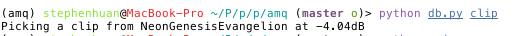
\includegraphics[scale=0.5]{clip.png}
      \caption{Generating a clip from an anime intro.}
    \end{subfigure}
    
    \begin{subfigure}[h]{0.4 \textwidth}
      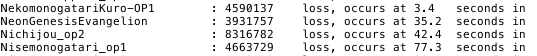
\includegraphics[scale=0.3]{compare.png}
      \caption{Comparison between songs; finds it occurs exactly 35.2 seconds in.}
    \end{subfigure}
    \hfill
    \begin{subfigure}[h]{0.4 \textwidth}
      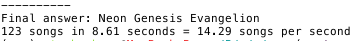
\includegraphics[scale=0.3]{result.png}
      \caption{Song with the lowest loss.}
    \end{subfigure}
    \caption{An example run of the system.}
\end{figure}
\end{frame}

\begin{frame}
\frametitle{Audio Information}
\framesubtitle{}
First, some basics about the representation of audio data. \pause

We will use the mp3 file format at a sample rate of 48kHz. \pause 

Audio is fundamentally just a list of numbers, where each number represents
the amplitude of the sound wave at that time. A 48kHz sample rate means 
there are 48,000 of these measurements per second. \pause

Each number is a 16-bit number in the range \( [0, 1) \), which we
will transform to an integer in the range \( [0, 2^{16}) \) for the NTT.
\end{frame}

\begin{frame}
\frametitle{Modeling the Problem}
\framesubtitle{}
So we have two lists of integers, and now wish to find where the smaller list
\enquote{fits} into the larger list the best. \pause

One way to do this is to compute the \alert{\( \ell^2 \) norm},
or the vector difference between the two lists. \pause

So we slide the smaller list over the larger list, computing the sum of squares
error as we go. Note that this is very similar to the convolution, except
we to calculate the sum of squares instead of the element-wise product.
We also need to flip one of the lists because the convolution flips a list.
\end{frame}

\begin{frame}
\frametitle{Turning Sum of Squares into Convolutions}
\framesubtitle{}
How do we reduce sum of squares to an element-wise product?
\pause
We notice that for elements of the lists \( a, b \)
\[ (a_i - b_j)^2 = a_i^2 - 2a_i b_j + b_j^2 \]
\pause 
When we sum over the length of \( a \),
assuming \( a \) is the smaller list, we get:
\[ \norm{a}^2 - 2 a \cdot b' + \norm{b'}^2 \] 
where \( b' \) is the slice that \( a \) overlaps.
\pause
\( \norm{a} \) is a constant, so it can be ignored.
Thus, we only need to compute \( a \cdot b' \) and \( \norm{b'} \).
\pause
\( a \cdot b' \) directly follows from a convolution and
can be read from \( a * b^r \), where \( b^r \) is the reverse of \( b \).
\pause
Lastly, if we make sure to scan from left to right, then we can compute
\( \norm{b'} \) by storing an intermediate value, and updating it when we slide 
\( a \) an additional index by subtracting out the front of \( b' \), where
\( a \) left from, and adding the new value that \( a \) covers.
\end{frame}

\begin{frame}[fragile]
\frametitle{Minimum \( \ell^2 \)}
\framesubtitle{}
\begin{algorithm}[H]
  \caption{minimum \( \ell^2 \) between two lists}
  \begin{minted}[frame=none, fontsize=\footnotesize]{python}
  def min_offset(a: list, b: list) -> tuple:
      N, M = len(a), len(b)
      p = fft(a[::-1], b)[N - 1:]
      x2, xy, y2 = sum(x*x for x in a), p[0], \
                   sum(b[i]*b[i] for i in range(N))
      best, l2 = 0, -2*xy + y2
      for i in range(1, M - N + 1):
          y2 += b[N - 1 + i]*b[N - 1 + i] - b[i - 1]*b[i - 1]
          xy = p[i]
          d = -2*xy + y2
          if d < l2:
              best, l2 = i, d
      return best, x2 + l2
  \end{minted}
\end{algorithm}
\end{frame}

\begin{frame}
\frametitle{NTT Considerations}
\framesubtitle{}
We need to be careful about a few things. If we don't pick \( p \) for the NTT
large enough, then it won't work. \pause

If \( m \) is the largest number in a list
and \( n \) is the length of the list, then we need \( p \) to be bigger than
\( m^2 n \), \\ the largest a single element can become. \pause

\( n \) is \( 90 \cdot 48,000 \approx 4 \cdot 10^6 \) and \( m \) is
\( 2^{16} \). \( m^2 n = 2^{32} \cdot 4 \cdot 10^6 \approx 2^{54} \). \pause

This seems fine since \( 2^{54} \) will fit in a long, but this won't work
since we need to compute \( x^2 \) as part of the FFT, and \( (2^{54})^2 \)
will definitely overflow. \pause

We could get around this overflow by doing modulo
multiplication instead of standard multiplication, but that would introduce
a log factor, making the algorithm 64x slower, an unacceptable slowdown.
\end{frame}

\begin{frame}
\frametitle{\( \mu \)-law Companding Algorithm}
\framesubtitle{}
One trick is to reduce the bitrate of the mp3 at the sacrifice of audio quality,
and go from 16-bit audio to 8-bit audio. \pause

A naive way to do it would be to multiply the real number by \( 2^8 \) and
round, but a better way is the \( \mu \)-law algorithm, a trick that preserves
frequencies closer to the human voice. A comparison between naive scaling
and the \( \mu \) law is presented
\href{https://www.youtube.com/watch?v=PqkE_t5cCoA}{here}. \pause

With 8-bit audio, \( m^2 n = 2^{16} \cdot 4 \cdot 10^6 \approx 2^{38} \).
This goes over the limit of \( 2^{32} \) for \( x^2 \) to fit in a long,
but it works in practice since mp3 audio rarely hits maximum volume and
our clip is 10 seconds long, and we computed for 90 seconds. \pause

An implementation is given
\href{https://github.com/stephen-huan/anime-music-quiz}{here} and a video
walkthrough \href{https://www.youtube.com/watch?v=7fUicc_lIGA}{here}.
\end{frame}

\subsection{2D Convolutions}
\begin{frame}
\frametitle{2D Convolutions}
\framesubtitle{}
2D convolutions, a convolution generalized to matrices, are useful in computer
vision for a variety of reasons, including edge detection and convolutional
neural networks. Their exact usage will not be discussed here, and instead
we will discuss an efficient way to calculate a 2D convolution with the FFT we 
have already developed. 

\begin{alertblock}{Definitions}
  We have an \enquote{data} matrix, representing an image,
  and we have a \emphasis{kernel} matrix, which is the matrix we imagine
  sliding over the image. This is also known as a \emphasis{filter}.
\end{alertblock}
\end{frame}

\begin{frame}
\frametitle{Scipy Definition}
\framesubtitle{}
For 2D convolutions, the result is slightly ambiguous \\
depending on how one defines it. 

We will use
\href{https://docs.scipy.org/doc/scipy/reference/generated/scipy.signal.convolve2d.html}{scipy's}
definition, where to calculate the value of the convolution at a particular
point, we imagine the \textit{bottom right} corner of the kernel
placed over that point.
\end{frame}

\begin{frame}
\frametitle{Convolution Example}
\framesubtitle{}
\begin{figure}[h!]
  \centering
  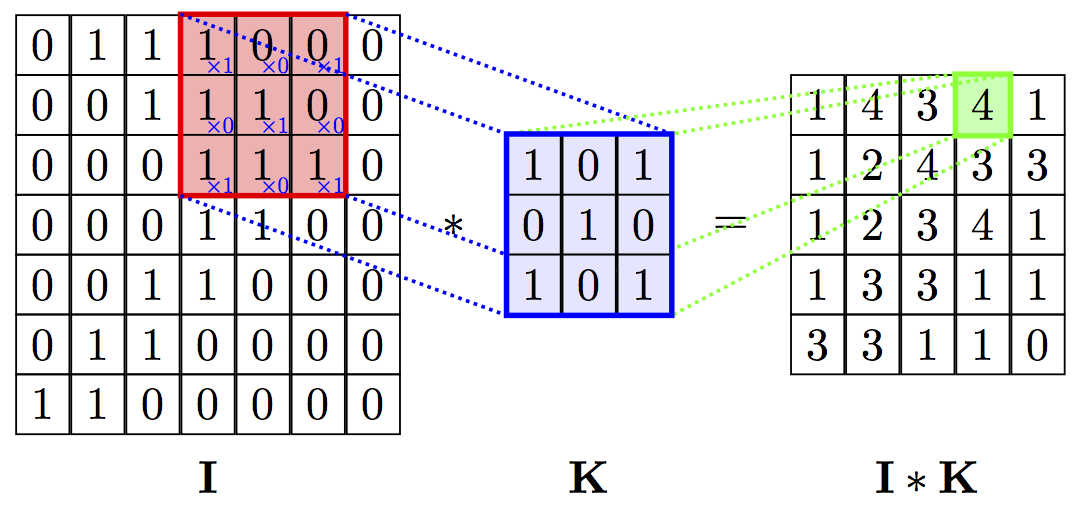
\includegraphics[scale=1]{conv.png}
  \caption{A convolution taken from \href{https://petar-v.com/GAT/}{here}.}
\end{figure}
\end{frame}

\begin{frame}
\frametitle{Definition of a 2D Convolution}
\framesubtitle{}
We define the 2D convolution between an image \( x \) of size \( M \)x\( N \)
and a kernel \( h \) of size \( H \)x\( W \) as follows
(similar to the 1D case, we assume both matrices are padded with 0's):
\begin{alertblock}{Definition of the 2D convolution}
  \[ (x * h)[i, j] = \sum^i_{k = 0} \sum^j_{l = 0} x[k][l]h[i - k][j - l] \]
\end{alertblock}
\end{frame}

\begin{frame}
\frametitle{}
\framesubtitle{}
This operation is also symmetric, so  what we call the image and the kernel
is essentially arbitrary (by convention, the kernel is the smaller matrix).
The resulting matrix is going to be of size \( (M + H - 1) \)x\( (N + W - 1) \)
from the same logic as the 1D case. \pause 

Thus, the time it takes to compute the convolution is \( O(MNHW) \).
We can, however, take advantage of a trick if the kernel has a certain property.
\end{frame}

\subsection{Separable Kernels}
\begin{frame}
\frametitle{Separable Kernels}
\framesubtitle{}
\begin{alertblock}{Separable}
  A matrix \( M \) is \emphasis{separable} if it can be written as
  \( \vec{u} \vec{v}^T \) for some vectors \( \vec{u}, \vec{v} \).
\end{alertblock}
\pause
\begin{exampleblock}{Sobel matrix}
  The famous Sobel matrix for edge detection is separable:
  \[
    \begin{bmatrix}
      1 & 0 & -1 \\
      2 & 0 & -2 \\
      1 & 0 & -1
    \end{bmatrix}
    =
    \begin{bmatrix}
      1 \\
      2 \\ 
      1
    \end{bmatrix}
    \begin{bmatrix}
      1 & 0 & -1
    \end{bmatrix}
  \]
\end{exampleblock}
\pause
\begin{block}{Separating the convolution}
  If \( M \) is separable, we can convolute with
  \( \vec{u} \) and then with \( \vec{v} \).
\end{block}
\end{frame}

\begin{frame}
\frametitle{Proof of Separability}
\framesubtitle{}
\only<1| handout:1>{
\begin{theorem}
  If \( h = \vec{u} \vec{v}^T \), then \( (x * h) = ((x * \vec{u}) * \vec{v}) \),
  i.e. we can separate a convolution into two parts.
\end{theorem}
}
\begin{proof}
  \begin{align*}
    \only<1| handout:1>{
    (x * u)[i, j] &= \sum^i_{k = 0} \sum^j_{l = 0} x[k][l]u[i - k][j - l] &&
    \text{Definition} \\
    \shortintertext{Since \( u \) is a column vector, it only has values when
    \( l = j \), removing the inner sum.}
                  &= \sum^i_{k = 0} x[k][j]u[i - k][0]
    }
    \only<2| handout:2>{
    \shortintertext{Convoluting with \( v \),}
    ((x * u) * v)[i, j] &= \sum^i_{k = 0} \sum^j_{l = 0} (\sum^k_{m = 0} x[m][l]u[k - m][0]) v[i - k][j - l] \\ 
    \shortintertext{Since \( v \) is a row vector, it only has values when
    \( k = i \), removing the outermost sum.}
                        &= \sum^j_{l = 0} (\sum^i_{m = 0} x[m][l]u[i - m][0]) v[0][j - l] \\ 
    }
    \only<3| handout:3>{
    \shortintertext{Swapping the order of summations and
    renaming \( m \) to \( k \),}
                        &= \sum^i_{k = 0} \sum^j_{l = 0} x[k][l]u[i - k][0] v[0][j - l] \\
    \shortintertext{From the fact that \(h[x][y] = u[x][0] v[0][y] \),}
                        &= \sum^i_{k = 0} \sum^j_{l = 0} x[k][l]h[i - k][j - l] \\
                        &= (x * h) \uncover<3>{\qedhere}
    }
  \end{align*}
\let\qedsymbol\relax
\end{proof}
\end{frame}

\begin{frame}
\frametitle{Runtime Analysis}
\framesubtitle{}
How does this help us? \pause

Well, recall the running time of \( O(MNHW) \).
If we do two convolutions of a kernel of \( H \)x1  and another of 1x\( W \),
the running time will be \( O(MNH + MNW) = O(MN(H + W)) \), a significant
improvement as \( HW \) grows quadratically while \( H + W \) grows linearly.
\pause

We can also use repeated 1D convolution to compute the 2D convolution for the
specific case of a vector, yielding a \( O(MN \log MN) \) time algorithm.
\end{frame}

\begin{frame}
\frametitle{}
\framesubtitle{}
However, not every matrix is separable. The conditions are quite strict,
a matrix is separable if and only if every pair of rows is a multiple of each
other, i.e. the matrix is made up of multiples of a particular row vector.
As a consequence, the matrix is also made up of multiples of a particular
column vector. These matrices are relatively rare, so there is utility
in deriving a more general algorithm.
\end{frame}

\subsection{FFT Algorithm}
\begin{frame}
\frametitle{Reduction to 1D Convolution}
\framesubtitle{}
We can reduce 2D convolutions to 1D convolutions if we're clever.
The observation is that if we \alert{flatten} both matrices into a 1D list
by reading from top to bottom, left to right, we can just convolute in 1D
and reconstruct the matrix afterwards. \pause

We need to make sure both matrices are sufficiently padded with zeros, such that
the zeros force values in the kernel to their proper rows in the image. \pause

It turns out that we can just pad both matrices
to the final column size of the convolution, 
\( N + W - 1 \), flatten both, convolute with the FFT, and then reshape the
resulting list to a matrix of proper size.
\end{frame}

\begin{frame}
\frametitle{Summary}
\framesubtitle{}
\begin{enumerate}[<+->]
  \item Pad the rows of both matrices with zeros such that
    each has a width of \( N + W - 1 \)
  \item Flatten both by reading top to bottom, left to right
  \item Convolute the resulting lists in 1D
  \item Reconstruct a 2D matrix, because we know its shape is
    \( (M + H - 1) \)x\( (N + W - 1) \)
\end{enumerate}
\end{frame}

\begin{frame}[fragile]
\frametitle{The 2D Convolution Algorithm}
\framesubtitle{}
\begin{algorithm}[H]
  \caption{2D Convolution Algorithm}
  \begin{minted}[frame=none]{python}
  def flatten(m: list, pad=0) -> list:
      """ Flattens a matrix into a list. """
      return [x for row in m for x in row + [0]*pad]

  def reshape(l: list, m: int, n: int) -> list:
      """ Shapes a list into a MxN matrix."""
      return [[l[r*n + c] for c in range(n)]
              for r in range(m)]

  def conv(h: list, x: list):
      """ Computes the 2D convolution. """
      M, N, H, W = len(x), len(x[0]), len(h), len(h[0])
      # need to pad the columns to the final size
      h, x = flatten(h, N - 1), flatten(x, W - 1)
      return reshape(fft(h, x), M + H - 1, N + W - 1)
  \end{minted}
\end{algorithm}
\end{frame}

\begin{frame}
\frametitle{Trimming}
\framesubtitle{}
In most computer vision applications, the kernel is a square matrix
of size \( K \)x\( K \), where \( K \) is an odd number. \pause

The \textit{middle value} of the kernel is then placed over each pixel of the
image, yielding a transformed image of the same dimensionality as the original.
\pause

We can simulate this by simply cutting off the first and last
\( \frac{K - 1}{2} \) rows and the same for the columns.
This transforms the resulting size from \( N + K - 1 \) to
\( N + K - 1 - 2 \frac{K - 1}{2} = N \).
\end{frame}

\begin{frame}[fragile]
\frametitle{Trimming}
\framesubtitle{}
\begin{minted}[label=pruning]{python}
def prune(h: list, x: list) -> list:
    """ Prunes a convolution for the specific KxK filter case. """
    m, k = conv(h, x), min(len(h), len(x))
    pad = (k - 1)>>1
    return [row[pad:-pad] for row in m[pad:-pad]]
\end{minted}
\end{frame}

\begin{frame}
\frametitle{Runtime Analysis}
\framesubtitle{}
The running time of the algorithm is going to be
\( O(MN \log MN) = O(MN(\log N + \log M) = O(MN \log N) \) since we convolute 
a list of length \( M(N + W - 1) \), and we assume \( N \geq M > W \). \pause

This is not necessarily faster than the brute-force algorithm;
it depends on the kernel size. For simplicity, suppose we have a \( N \)x\( N \)
image and a \( K \)x\( K \) kernel where \( N > K \). Brute force yields
\( O(N^2 K^2) \) while the FFT algorithm yields \( O(N^2 \log N) \). \pause

Thus, if \( \log N < K^2 \) then the FFT algorithm is going to be faster.
For \( K > 5 \) that is a fair assumption since \( K^2 = 25 \), \( 2^{25} \)
is several million. Obviously the FFT algorithm has a much larger constant
factor, but for a sufficiently large kernel the time savings become greater
and greater.
\end{frame}

\section{Conclusion}

\begin{frame}
\frametitle{Conclusion}
\framesubtitle{}
The convolution, an operator very useful for signal, audio, and image
processing, can be efficiently computed with the Fast Fourier Transform, or FFT.
\pause

If the data is integer, then floating-point arithmetic can be avoided with the
Number Theoretic Transform (NTT), a variant of the FFT which uses modulo
instead of complex numbers, and calculates entirely in integers.
\end{frame}

\begin{frame}
\frametitle{Conclusion}
\framesubtitle{}
This lecture skips over the continuous case (what I've been calling the 
Fast Fourier Transform is more mathematically called the
\alert{Discrete Fourier Transform}, or DFT) but the idea is essentially the
same, any summation turns into an integral. \pause

It also skips over the mathematical interpretation of the FFT,
involving decomposing a function into a series of sine and cosine waves.
This is useful for signal processing and audio analysis,
but requires a stronger mathematical background and to be honest, I haven't
studied it at all myself. Fourier analysis goes deeper than we need here. 
\end{frame}

\begin{frame}
\frametitle{Conclusion}
\framesubtitle{}
\textit{Introduction to Algorithms} is definitely the most helpful source on
the FFT (from a computer science perspective), and more thorough treatments of
the FFT from an engineering or mathematical standpoint are not hard to find.
\end{frame}

\section{Sample Problems}
\begin{frame}
\frametitle{Sample Problems}
\framesubtitle{Examples of problems using the FFT}
\begin{enumerate}[<only@+| handout:only@+>]
  \item \href{https://www.spoj.com/problems/POLYMUL/}{SPOJ POLYMUL}:
    Direct application of the FFT.

  \item \href{https://www.spoj.com/problems/MUL/}{SPOJ MUL}:
    Given 1000 pairs of numbers, compute the product of each pair;
    each number can have up to 10,000 digits.
    \addtocounter{enumi}{-1}
  \item Solution: Think of numbers as polynomials,
    where the digits are coefficients and \( x \) is 10.
    Then, you can multiply two numbers by multiplying the polynomials.
    However, there is no guarantee that the coefficients
    of the resulting polynomial are less than 10, so it is not a valid number.
    As a last post-processing step, start from the smallest place value
    and move your way to the largest, moving the digit overflow from one place
    value to the next. Since you iterate over the number of digits in the
    number, it takes \( O(\log n) \) which is dominated by the FFT.  
    \addtocounter{enumi}{-1}
  \item An extension of this idea is the 
    \href{https://en.wikipedia.org/wiki/Sch\%C3\%B6nhage\%E2\%80\%93Strassen_algorithm}
    {Schönhage–Strassen} algorithm, which disregards the requirement
    that the intermediate numbers fit in a long, at the cost of being
    \( O(n \log n \log \log n) \). A more recent algorithm,
    by Harvey and van der Hoeven, achieves 
    \href{https://hal.archives-ouvertes.fr/hal-02070778/document}{\( O(n \log n) \)}.

  \item \href{https://www.spoj.com/problems/MAXMATCH/}{SPOJ MAXMATCH}:
    Given a string \( S \) of length \( N \) made up of the characters
    \enquote{a}, \enquote{b}, and \enquote{c}, compute the maximum
    self-matching, where a self-matching is defined as the number of characters
    which match between \( S \) and \( S \) shifted some
    nonzero number of characters.
   \addtocounter{enumi}{-1}
 \item Solution: For an offset \( i \), the size of the overlap
    will be \( N - i \). So we just need to find the number of differences,
    and subtract that from \( N - i \) to obtain the number of matches.
    The easiest thing to do is to keep track of each character separately,
    so to compute the differences for each character.
    Suppose our character is \enquote{a}. We encode \enquote{a} as a 0,
    and the other characters as a 1. We then find the \( \ell^2 \) norm between 
    this new list and this list with \( N \) 1's added to it
    (so that when we overlap, the non \enquote{a} characters aren't counted).
    This has the complication of counting \enquote{a}'s which are off the edge
    of the string, which we can account for by simply keeping track of the 
    number of \enquote{a}'s we have seen.
    \addtocounter{enumi}{-1}
  \item Given \( a[i] \) as the number of mismatches with the character \enquote{a}
    at a shift of \( i \), and \( b[i], c[i] \), the number of matches is 
    \( N - i - \frac{a[i] + b[i] + c[i]}{2} \). We divide by 2 because we
    count each mismatch twice (once for each character in the pair).
    \addtocounter{enumi}{-1}
  \item A much conceptually simpler algorithm is to encode \enquote{a}, \enquote{b},
    and \enquote{c} cleverly and then compute the matches in one shot. 
    If we encode \enquote{a} as (1, 0, 0), \enquote{b} as (0, 1, 0), and
    \enquote{c} as (0, 0, 1), the FFT of the resulting list with its reverse
    will give us the number of matches at each index because the character
    representations dot each other will be 1 if they are equal, and 0 
    if they are unequal. Thus, the FFT will give us exactly the number of
    matches, but we need to only look at every 3rd index since the other 2
    are byproducts of our transformation.

    In practice, running one big FFT is faster than running 3 smaller FFTs.

  \item \href{https://www.codechef.com/problems/FARASA}{Codechef FARASA}:
    Given an array, find the number of distinct sums of a contiguous subarray.
    \addtocounter{enumi}{-1}
  \item Solution: \href{https://discuss.codechef.com/t/farasa-editorial/2688}
    {editorial}.

    Fair warning, time bounds are ridiculous.

  \item \href{https://codeforces.com/contest/528/problem/D}
    {Codeforces Round \#296}: Given two strings \( T, S \) and 
    an error bound \( k \), find all the positions where \( T \) occurs
    in \( S \), where \( T \) \enquote{occurring} at some index \( i \) 
    means that the \( j \)th character of \( T \) has a corresponding character
    within \( k \) of its position.
    \addtocounter{enumi}{-1}
  \item Solution: Honestly no clue but it has the \enquote{FFT} tag.

  \item \href{https://cs.stanford.edu/~rishig/courses/ref/l17.txt}
    {String matching with wildcards}: Given two binary strings \( T, S \),
    \( T \) has length \( N \) and has wildcards which match any character
    in \( S \), find all occurrences of \( T \) in \( S \).
    \addtocounter{enumi}{-1}
  \item Solution: Encode 1 as 1 and 0 as -1. The dot product between \( T \)
    and the slice that \( T \) overlaps with \( S \) will be be \( N \)
    if they match exactly and less than \( N \) if they don't match exactly.
    To account for wildcards, encode a wildcard as \( 0 \) and count the
    number of wildcards, \( C \). Then, if they match exactly it will be
    \( N - C \), and less then that if they don't.
    \addtocounter{enumi}{-1}
  \item This can be generalized to non-binary strings if you apply the above
    algorithm to each character, setting that character as 1 and not that
    character as -1. Sum over all possible characters, and that will tell you
    whether there is a mismatch somewhere (similar to SPOJ MAXMATCH).
    \addtocounter{enumi}{-1}
  \item This idea can also be applied to string matching without wildcards.
    Encode each character as its ASCII value in a polynomial, and compute
    the \( \ell^2 \)-norm between \( T \) and \( S \). The \( \ell^2 \) norm
    will be 0 if they match, and positive if they don't.

  \item \href{https://en.wikipedia.org/wiki/3SUM}{3SUM}:
    Given a list of integers between \( -N \) and \( N \),
    find 3 numbers that add up to 0 (duplicates are allowed). 
    \addtocounter{enumi}{-1}
  \item Solution: The basic idea will be to encode the list into a length \( 2N \)
    polynomial \( p \) where the degree is an integer value and the coefficient
    is whether that value appears in the array.
    Compute \( p^3 \) and read off the coefficient of \( x^0 \).
    \addtocounter{enumi}{-1}
  \item However, this doesn't work if the degrees are negative. If the most
    negative power of \( x \) in \( p \) is \( x^{-N} \), We can simply multiply
    \( p \) by \( x^N \) to make every power positive, making a new polynomial
    \( p' \). Then, after computing \( (p')^3 \), instead of looking at the
    coefficient of \( x^0 \), we can look at the coefficient of \( x^{-3N} \)
    (accounting for the fact that \( p' = x^N p \), \( (p')^3 = x^{3N} p^3 \),
    \( p^3 = \frac{(p')^3}{x^{3N}} \)
    \addtocounter{enumi}{-1}
  \item Alternative solution, if duplicates aren't allowed:
    \href{https://cs.stanford.edu/~rishig/courses/ref/l16.txt}{here}
    (look for \enquote{color coding}).

  \item \href{https://animemusicquiz.com/}{Anime Music Quiz}:
    Guess which anime an intro/outro comes from.
    \addtocounter{enumi}{-1}
  \item Solution: The \href{https://www.toptal.com/algorithms/shazam-it-music-processing-fingerprinting-and-recognition}
    {Shazam algorithm}.
\end{enumerate}
\end{frame}

\section{Past Lectures}

\begin{frame}
\frametitle{Past Lectures}
\framesubtitle{Past Lectures on similar topics}
\begin{enumerate}
  \item \href{https://activities.tjhsst.edu/computervision/lectures/Edge_Detection.pdf}
    {\enquote{Edge Detection}}, (Alexey Didenkov, 2018)
  \item \href{https://activities.tjhsst.edu/sct/lectures/1516/SCT_Polynomial.pdf}
    {\enquote{Fast Multiplication: Karatsuba and FFT}} (Haoyuan Sun, 2016)
  \item \href{https://activities.tjhsst.edu/sct/lectures/1415/SCT_Multiplying_Polynomials.pdf}
    {\enquote{Multiplying Polynomials}}, (Haoyuan Sun, 2015)
  \item \href{https://activities.tjhsst.edu/sct/lectures/1213/fft.pdf}
    {\enquote{Fast Fourier Transform}}, (Sreenath Are, 2013)
\end{enumerate}
\end{frame}

\section{References}
\begin{frame}
\frametitle{References}
\framesubtitle{Resources that were useful when compiling this lecture}
\begin{enumerate}
  \item \href{https://mitpress.mit.edu/books/introduction-algorithms-third-edition}
    {\textit{Introduction to Algorithms}}, chapter 30 (very helpful)
  \item \href{https://www.nayuki.io/page/number-theoretic-transform-integer-dft}
    {The number theoretic transform}
  \item \href{https://en.wikipedia.org/wiki/\%CE\%9C-law_algorithm}
    {\( \mu \)-law algorithm}
  \item \href{https://ptolemy.berkeley.edu/projects/embedded/eecsx44/lectures/Spring2013/Picard.pdf}
    {Picard's Existence and Uniqueness Theorem}
  \item \href{https://towardsdatascience.com/a-basic-introduction-to-separable-convolutions-b99ec3102728}
    {Separable convolutions}
\end{enumerate}
\end{frame}

\end{document}
